% Preamble
\documentclass[11pt]{article}
\usepackage{perf}

% Document
\begin{document}

    \perfset{
    robust fast \\
    5    30 \\
    2     1 \\
    2     1 \\
    5    50 \\
    5     1 \\
    2     1 \\
    2     1 \\
    4     1 \\
    2     1 \\
    3     1 \\
    4    45 \\
    }

    \printperftable

    \vspace{1cm}
    \begin{tikzpicture}
        \begin{axis}[title=Performances,height=6cm]
            \addperformances
            \legend{robust, fast}
        \end{axis}
    \end{tikzpicture}

    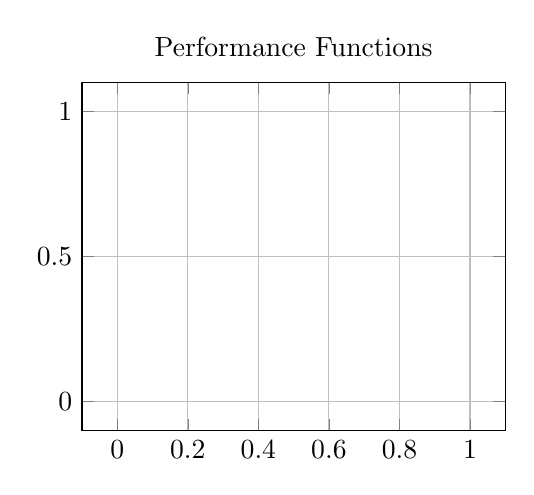
\begin{tikzpicture}
        \begin{axis}[title=Performance Functions,height=6cm,
        legend pos=outer north east,grid=both,no marks]
            \addprofiles
            \legend{robust,fast}
        \end{axis}
    \end{tikzpicture}


    %
    % Second set of data and plots
    %

    \perfset{
    better worse \\
    1    30 \\
    1     2 \\
    1     3 \\
    1    50 \\
    1     3 \\
    1     2 \\
    30     1 \\
    }

    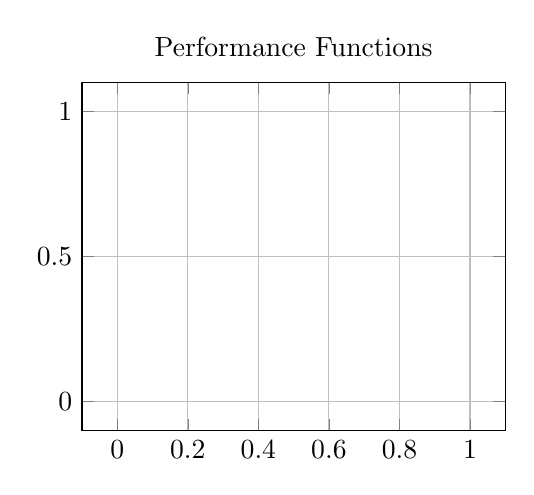
\begin{tikzpicture}
        \begin{axis}[title=Performance Functions,height=6cm,
        legend pos=outer north east,grid=both,no marks]
            \addprofiles
            \legend{better,worse}
        \end{axis}
    \end{tikzpicture}


\end{document}